\section{شمارنده‌ها}
\begin{frame}{چرا شمارنده‌ها}
\begin{itemize}\itemr
\item[-]
در نوشتن متون، مواقعی پیش می‌آید که باید به تعداد مشخص یا نامشخصی مواردی را بنویسیم و برای آنها شماره‌گذاری انجام دهیم،

\item[-]
مثل ردیف جدول‌ها.

\item[-]
اما انجام دادن دستی این کار، عدم دقت، ناهماهنگی و زحمت زیادی را برای ما دارد.

\item[-]
راهکار نرم‌افزار لاتک، استفاده از شمارنده‌هاست.
\end{itemize}
\end{frame}

\begin{frame}{استفاده‌ی خود لاتک از شمارنده‌ها}
\begin{itemize}\itemr
\item[-]
لاتک برای شماره‌گذاری صفحات، قسمت‌ها، فصول و سکشن‌ها
(\ref{parts-chapters})،
 و موارد زیاد دیگری از شمارنده‌های درونی خودش استفاده می‌کند.
\end{itemize}
\end{frame}

\begin{frame}[fragile]{نمونه کد}
\begin{latin}
\begin{lstlisting}[keywords={begin, end}, keywordstyle=\color{Mulberry}\textbf]
\LaTeX uses counters for
\begin{enumerate}
    \item \textbackslash part
    \item \textbackslash chapter
    \item \textbackslash section
    \item \textbackslash subsection
\end{enumerate}
\end{lstlisting}
\end{latin}
\end{frame}

\begin{frame}{خروجی}
\begin{center}
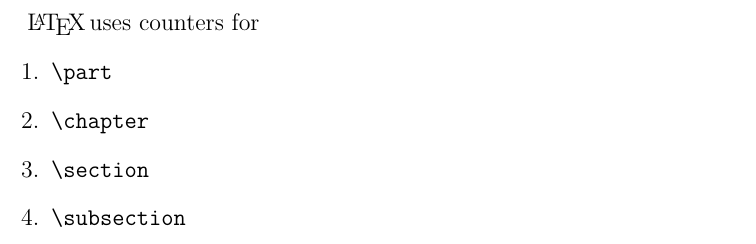
\includegraphics[width=\textwidth]{docs/images/enum-1}
\end{center}
\end{frame}

\begin{frame}[fragile]{نمونه کد}
\begin{latin}
\begin{lstlisting}[keywords={begin, end}, keywordstyle=\color{Mulberry}\textbf]
\LaTeX uses counters for
\begin{enumerate}
    \item even this \texttt{enumerate} environment
    \item \textbackslash part
    \item \textbackslash chapter
    \item \textbackslash section
    \item \textbackslash subsection
\end{enumerate}
\end{lstlisting}
\end{latin}
\end{frame}

\begin{frame}{خروجی}
\begin{center}
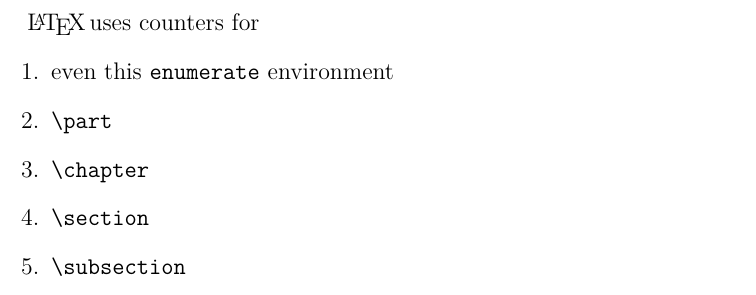
\includegraphics[width=\textwidth]{docs/images/enum-2}
\end{center}
\end{frame}


\begin{frame}{تعریف شمارنده}
\begin{itemize}\itemr
\item[-]
برای تعریف شمارنده‌های باید از دستور
\lr{\texttt{\textbackslash newcounter\{NameOfCounter\}}} 
استفاده کرد.
\end{itemize}
\end{frame}

\begin{frame}{تعریف شمارنده}
\begin{itemize}\itemr
\item[-]
برای دسترسی به مقدار شمارنده، از این سه روش می‌توان استفاده کرد:

\begin{enumerate}\itemr
\item 
\lr{\texttt{\textbackslash theNameOfCounter}}

\item 
\lr{\texttt{\textbackslash value\{NameOfCounter\}}}

\item
\lr{\texttt{\textbackslash arabic\{NameOfCounter\}}}
\end{enumerate}
\end{itemize}
\end{frame}

\begin{frame}{حالت مقدار شمارنده}
\begin{itemize}\itemr
\item[-]
\lr{\texttt{\textbackslash arabic}}

برای مقادیر $-2^{31}$ تا $2^{31}$

\item[-]
\lr{\texttt{\textbackslash alph}}

به ترتیبِ حروف الفبا در انگلیسی و حروف ابجد در فارسی

\item[-]
\lr{\texttt{\textbackslash roman}}

حروف یونانی
\end{itemize}
\end{frame}

\begin{frame}{عدد دهی به شمارنده و گام شمارنده}
\begin{itemize}\itemr
\item[-]
برای مقداردهی به شمارنده (چه به صورت پیشفرض به عدد صفر مقداردهی می‌شوند) از دستور 
\lr{\texttt{\textbackslash setcounter\{NameOfCounter\}\{number\}}}
استفاده می‌شود.

\item[-]
برای گامِ شمارنده، از دستور 
\lr{\texttt{\textbackslash stepcounter\{NameOfCounter\}}}
استفاده می‌شود.
\end{itemize}
\end{frame}

\begin{frame}[fragile]{نمونه کد}
\begin{latin}
\begin{lstlisting}[keywords={begin, end}, keywordstyle=\color{Mulberry}\textbf]
\newcounter{record}
\begin{table}[h]
\begin{tabular}{|c|c|}
\hline
record & course \\
\hline
\hline
\stepcounter{record}\arabic{record} & Operating System \\
\hline
\stepcounter{record}\arabic{record} & Computer Networks \\
\hline
\stepcounter{record}\arabic{record} & Signals and Systems \\
\hline
\stepcounter{record}\arabic{record} & Project Management \\
\hline
\end{tabular}
\end{table}
\end{lstlisting}
\end{latin}
\end{frame}

\begin{frame}{خروجی}
\begin{center}
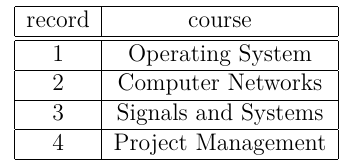
\includegraphics[width=0.5\textwidth]{docs/images/engcounter}
\end{center}
\end{frame}

\begin{frame}{خروجی}
\begin{center}
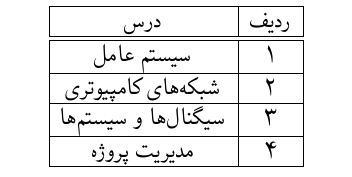
\includegraphics[width=0.5\textwidth]{docs/images/facounter}
\end{center}
\end{frame}
